% Copyright (c) 2026 CorrectBrain
% SPDX-License-Identifier: MIT

\PassOptionsToPackage{dvipsnames,svgnames,x11names}{xcolor}
\documentclass[tikz,border=8pt]{standalone}
\usetikzlibrary{arrows.meta,positioning,calc,shapes,shadows,decorations.pathmorphing,shapes.geometric,backgrounds,decorations.markings,decorations.pathreplacing,decorations.text,fit,shapes.misc,shapes.arrows,matrix,bending,3d,chains,intersections,shapes.symbols,svg.path,shapes.multipart,snakes,shapes.callouts,angles,quotes}
\providecolor{gold}{RGB}{212,175,55}
\providecolor{silver}{RGB}{192,192,192}
\providecolor{bronze}{RGB}{205,127,50}
\providecolor{darkblue}{RGB}{0,0,139}
\providecolor{lightblue}{RGB}{173,216,230}
\providecolor{darkgreen}{RGB}{0,100,0}
\providecolor{lightgreen}{RGB}{144,238,144}
\providecolor{darkred}{RGB}{139,0,0}
\providecolor{navy}{RGB}{0,0,128}
\providecolor{skyblue}{RGB}{135,206,235}
\providecolor{beige}{RGB}{245,245,220}
\providecolor{cream}{RGB}{255,253,208}
\usepackage{amsmath}
\usepackage{amssymb}
\usepackage{fontawesome5}
\usetikzlibrary{fadings,shadows.blur,patterns,patterns.meta}
\usepackage{amsmath}
\usepackage{amssymb}
\usepackage{fontawesome5}
\usepackage{tikz}
\usepackage{xcolor}


\pagecolor{white}

% --- DEFINE CUSTOM COLORS ---
\definecolor{cssblue}{RGB}{41, 101, 241}
\definecolor{htmlorange}{RGB}{227, 79, 38}
\definecolor{enginepurple}{RGB}{123, 31, 162}
\definecolor{warnred}{RGB}{211, 47, 47}
\definecolor{darkgray}{RGB}{50, 50, 50}

\begin{document}
\sffamily
\begin{tikzpicture}

% --- TITLE & SUBTITLE ---
\node[font=\Huge\bfseries\color{darkgray}, anchor=center] at (-1.7, 15) {The Rendering Pipeline: Box vs. Payload Projection};
\node[font=\Large\color{gray}, anchor=center] at (-1.7225,13.5487) {How \texttt{object-fit} maps arbitrary physical intrinsic data into the algorithmically constrained \texttt{aspect-ratio} box};

% ==========================================
% STEP 1: THE CSS BOX
% ==========================================
\node[anchor=north west, inner sep=0pt, text width=7.5cm] at (-9.5179,10.8741) {
    {\Large\bfseries\color{cssblue} 1. The Layout Box (16:9)}\\[6pt]
    {\normalsize\color{black!80} Constructed solely from CSS algorithms \texttt{width: 100\%} and \texttt{aspect-ratio: 16 / 9}. Exists independently of image content in the layout tree.}
};

% Box 16:9 -> Width 8, Height 4.5. (Coordinates: (-1, 7.25) to (7, 11.75))
\filldraw[fill=cssblue!5, draw=cssblue, ultra thick, dashed, rounded corners=2pt, pattern=grid, pattern color=cssblue!15] (-1, 7.25) rectangle (7, 11.75);

% Semantic Pill Badge (Resting on top of box)
\node[anchor=south west, fill=cssblue, text=white, font=\footnotesize\bfseries, rounded corners=3pt, inner sep=3.5pt] at (-1, 11.75) {DOM Layer};

% Box Label with solid white backing
\node[font=\Large\bfseries\color{cssblue}, fill=white, rounded corners=2pt, inner sep=4pt] at (3, 9.5) {Structural CSS Box};

% Measurement Indicators
\draw[<->, thick, cssblue] (-1, 6.6) -- (7, 6.6) node[midway, below, font=\bfseries] {$W$ (100\%)};
\draw[<->, thick, cssblue] (7.6, 7.25) -- (7.6, 11.75) node[midway, right, font=\bfseries] {$H = W \times \frac{9}{16}$};


% ==========================================
% STEP 2: THE PHYSICAL PAYLOAD
% ==========================================
\node[anchor=north west, inner sep=0pt, text width=7.5cm] at (-9.5179,5.3458) {
    {\Large\bfseries\color{htmlorange} 2. The Intrinsic Payload (4:3)}\\[6pt]
    {\normalsize\color{black!80} The physical image bytes received over the network. It has its own unchangeable intrinsic aspect ratio dictated by the camera/creator (e.g. 4000x3000px).}
};

% Box 4:3 -> Width 6, Height 4.5. (Coordinates: (0, 1.25) to (6, 5.75))
\filldraw[fill=htmlorange!15, draw=htmlorange, ultra thick, rounded corners=2pt, blur shadow={shadow opacity=20, shadow yshift=-2pt}, pattern=crosshatch dots, pattern color=htmlorange!30] (0, 1.25) rectangle (6, 5.75);

% Semantic Pill Badge (Resting on top of box)
\node[anchor=south west, fill=htmlorange, text=white, font=\footnotesize\bfseries, rounded corners=3pt, inner sep=3.5pt] at (0, 5.75) {Raster Asset};

% Box Label with solid white backing
\node[font=\Large\bfseries\color{htmlorange!80!black}, fill=white, rounded corners=2pt, inner sep=4pt] at (3, 3.5) {\faCamera \quad Raster Image Data};

% Measurement Indicators
\draw[<->, thick, htmlorange] (0, 0.6) -- (6, 0.6) node[midway, below, font=\bfseries] {Intrinsic Width (4 units)};
\draw[<->, thick, htmlorange] (6.6, 1.25) -- (6.6, 5.75) node[midway, right, font=\bfseries] {Intrinsic Height (3 units)};


% ==========================================
% TRANSFORMATION PIPELINE
% ==========================================
% Nodes
\node[font=\Large\bfseries\color{enginepurple}, fill=white, inner sep=6pt, rounded corners=4pt, anchor=center] (matrixNode) at (3, -1.5) {\texttt{object-fit: cover} Transformation Matrix};

\node[anchor=center, draw=enginepurple!40, fill=white, rounded corners=4pt, inner sep=6pt, font=\small, blur shadow={shadow opacity=10, shadow yshift=-1pt}] (mathNode) at (3, -4.0) {$\text{Scale} = \max\left(\frac{W_{\text{box}}}{W_{\text{img}}}, \frac{H_{\text{box}}}{H_{\text{img}}}\right) = \max\left(\frac{8}{6}, \frac{4.5}{4.5}\right) = 1.33\times$};

% Arrows (Zero Collision Routing)
\draw[-Stealth=3mm, line width=1.5pt, enginepurple, shorten >=4pt, shorten <=4pt] (3, 1.25) -- (matrixNode.north);
\draw[-Stealth=3mm, line width=1.5pt, enginepurple, shorten >=4pt, shorten <=4pt] (matrixNode.south) -- (mathNode.north);
\draw[-Stealth=3mm, line width=1.5pt, enginepurple, shorten >=4pt, shorten <=4pt] (mathNode.south) -- (3, -7.0);


% ==========================================
% STEP 3: THE PROJECTION PIPELINE
% ==========================================
\node[anchor=north west, inner sep=0pt, text width=7.5cm] at (-11, -7) {
    {\Large\bfseries\color{enginepurple} 3. The Final Paint Projection}\\[6pt]
    {\normalsize\color{black!80} The browser's graphics layer scales the payload uniformly to cover the structural box, mathematically discarding (clipping) the spatial mismatch. \textbf{Layout remains entirely untouched!}}
};

% Scaled Image bounds: (-1, -13) to (7, -7)
% Layout Box bounds: (-1, -12.25) to (7, -7.75)

% 1. Clipped visible region (In-bounds viewport)
\begin{scope}
    \clip (-1, -12.25) rectangle (7, -7.75);
    \filldraw[fill=htmlorange!20, draw=htmlorange, ultra thick, pattern=crosshatch dots, pattern color=htmlorange!30] (-1, -13) rectangle (7, -7);
    \node[font=\Large\bfseries\color{htmlorange!80!black}, fill=white, rounded corners=2pt, inner sep=4pt] at (3, -10) {\faImage \quad Scaled Physical Pixels};
\end{scope}

% 2. Frosted/Dimmed Y-Axis Overflow Culling Regions
% Top Overflow: (-1, -7.75) to (7, -7)
\fill[white, opacity=0.75] (-1, -7.75) rectangle (7, -7);
\draw[warnred, ultra thick, dashed, pattern=north west lines, pattern color=warnred!40] (-1, -7.75) rectangle (7, -7);
\node[font=\small\bfseries\color{warnred}, fill=white, rounded corners=2pt, inner sep=2pt, anchor=center] at (3, -7.375) {Y-Axis Overflow Clipped};

% Bottom Overflow: (-1, -13) to (7, -12.25)
\fill[white, opacity=0.75] (-1, -13) rectangle (7, -12.25);
\draw[warnred, ultra thick, dashed, pattern=north west lines, pattern color=warnred!40] (-1, -13) rectangle (7, -12.25);
\node[font=\small\bfseries\color{warnred}, fill=white, rounded corners=2pt, inner sep=2pt, anchor=center] at (3, -12.625) {Y-Axis Overflow Clipped};

% 3. Overlay the CSS Layout Box boundaries
\draw[ultra thick, cssblue, dashed, rounded corners=2pt] (-1, -12.25) rectangle (7, -7.75);
\node[font=\small\bfseries\color{cssblue}, fill=white, rounded corners=2pt, inner sep=2pt, anchor=south west] at (-1, -12.25) {Layout Engine Boundary};

% Semantic Pill Badge (Resting on top of projection box)
\node[anchor=south west, fill=enginepurple, text=white, font=\footnotesize\bfseries, rounded corners=3pt, inner sep=3.5pt] at (-1, -7.0) {GPU Paint Layer};


% ==========================================
% BOTTOM CONCLUSION SECTION
% ==========================================
\node[anchor=north, draw=enginepurple, fill=enginepurple!5, rounded corners=8pt, text width=18cm, inner sep=15pt, blur shadow={shadow opacity=20}] at (-1.7, -15.0) {
    \textbf{\Large\color{enginepurple}\faCrop \quad Architectural Independence}\\[6pt]
    {\normalsize\color{black!80} By utilizing \texttt{aspect-ratio} paired with \texttt{object-fit}, the \textbf{DOM Layout phase} is mathematically severed from the \textbf{Paint/Render phase}. The structural HTML container is guaranteed stable by the layout engine (preventing CLS), while the GPU graphics hardware projects the network payload into the predefined coordinates during the Paint phase, seamlessly clipping any aspect ratio inconsistencies.}
};

\end{tikzpicture}
\end{document}
